\chapter{Light Propagation in Linear Isotropic Dielectrics	}
\section{Constitutive Equation for LInear Isotropic Dielectrics}
Précédemment\footnote{La page précédente quoi}, nous avions introduit une relation constitutive décrivant les
propriétés d'un matériau homogène et stationnaire
	\begin{equation}
	\begin{array}{ll}
	\DS P_i^{(n)}(r,t) =\epsilon_0&\DS\iiint_{V_0}dr_1\dots \iiint_{V_0} dr_n \int_{-\infty}^
	\infty dt_1\int_{-\infty}^	\infty dt_n\\
	&\DS \chi_{ij_1\dots j_n}^{(n)}(r-r_1,\dots,r-r_n,t,\dots,t-t_n)E_{j_1}(r_1,t_1)\dots
	E_{j_n}(r_n,t_n)
	\end{array}
	\end{equation}
Cette relation compliquée se simplifie avec les deux hypothèses suivantes
\begin{enumerate}
\item \textbf{Linéaire}. Les champs $\vec E, \vec{B}$ dépendent linéairement des termes sources $\rho,\vec P$ 
et $\vec M$. Linéaire signifie également qu'une combili de solutions est solution. 
\item \textbf{Isotropique}. Les relations entre $\vec E, \vec{B}$ et $\rho,\vec P, \vec M$ sont indépendantes
de la direction d'espace.
\end{enumerate}\ 
	
La première hypothèse ne laisse place qu'au terme du premier ordre
\begin{equation}
P_i(r,t) = \epsilon_0\iiint_{V_0} dr_1\int_{-\infty}^\infty dt_1\chi_{ij}^{(1)}(r-r_1,t-t_1)E_j(r_1,t_1)
\end{equation}
La seconde implique que le champ de polarisation doit être parallèle au champ électrique
\begin{equation}
P_i(r,t) = \epsilon_0\iiint_{V_0} dr_1\int_{-\infty}^\infty dt_1\chi^{(1)}(r-r_1,t-t_1)E(r_1,t_1)
\end{equation}
Etant une intégrale de convolution, elle se traite facilement dans le domaine des fréquences
\begin{equation}
E(k,\omega) = \iiiint E(r,t)e^{-i(wt-k. r)}drdt,\qquad E(r,t) = \frac{1}{(2\pi)^4}\iiiint E(k,\omega)e^{
i(\omega t-k.r)}dkd\omega
\end{equation}\ 

\cadre{La relation constitutive dans le domaine des fréquences devient alors
\begin{equation}
P(k,\omega) = \epsilon_0\chi(k,\omega)E(k,\omega)
\end{equation}
où il est clair qu'une interaction non-locale (non-instantanée) donne lieu à de la dispersion temporelle
(spatiale).}\ \\

\newpage
Les hypothèses
\begin{itemize}
\item[$\bullet$] \textbf{Causalité}. Susceptibilité nulle $\forall t < t_1$. Dans le domaine fréquentiel, elle fourni une 
relation entre la partie réelle et complexe de la susceptibilité.
\item[$\bullet$] \textbf{Instantané}. $\rho,\vec P,\vec J, \vec M$ ne dépendent que de $\vec E, \vec B$ au même instant.
\item[$\bullet$] \textbf{Local}. $\rho,\vec P,\vec J, \vec M$ ne dépendent que de $\vec E, \vec B$ au même point.
\end{itemize}
S'expriment
\begin{equation}
\chi^{(1)}(r-r_1,t-t_1)= \chi\delta(r-r_1,t-t_1)
\end{equation}
Ce qui implique
\begin{equation}
P(r,t) = \epsilon_0\chi E(r,t)
\end{equation}
Ce qui est une bonne approximation à basse fréquence\footnote{La TF d'une fonction réelle est complexe, la 
dispersion et l'atténuation sont liés.} et pour les matériaux transparents\footnote{Pas d'atténuation et donc 
pas de dispersion : interaction instantanée des dipôles.}


\section{Propagation of Plane Monochromatic Waves}
La relation constitutive linéaire simplifie les équations de Maxwell : $\vec{D}$ est linéaire en $\vec{E}$
\begin{equation}
D\equiv \epsilon_0+P = \epsilon_0(1+\chi)E = \epsilon E
\end{equation}
où $\epsilon = \epsilon_0(1+\chi)$. On en tire
\begin{equation}
\vec\nabla .\vec E = 0, \qquad\vec\nabla .\vec B = 0,\qquad \rot\vec{E} = -\frac{\partial\vec{B}}{\partial t}, 
\qquad\rot\vec{B} = \epsilon\mu_0\frac{\partial \vec{E}}{\partial t}
\end{equation}
Ce qui mène à l'équation d'onde bien connue
\begin{equation}
\Delta E - \epsilon\mu_0\frac{\partial^2 E}{\partial t^2}=0
\end{equation}
Possédant comme solution $E(r,t) = E_0\Re\left(e^{i\omega t-k.r)}\right)$. Par substitution de la solution, 
on trouve la \textbf{relation de dispersion}
\begin{equation}
k^2_x+k^2_y+k^2_z = \epsilon\mu\omega^2
\end{equation}
Qui devient $k_0=\sqrt{\epsilon_0\mu_0}$ dans le vide. On en déduit que la vitesse de la lumière dans le 
vide est donnée par $c=\omega/k_0 = 1/\sqrt{\epsilon_0\mu_0}$. La relation de dispersion dans un diélectrique 
est
\begin{equation}
k = \omega\sqrt{\epsilon\mu_0}
\end{equation}
On définit alors la \textbf{vitesse de phase} $v_\varphi = \omega/k = 1/\sqrt{\epsilon\mu_0}$. L'\textbf{indice
de réfraction} est défini comme le rapport entre la vitesse de la lumière sur la vitesse de phase
\begin{equation}
n = \dfrac{c}{v_\varphi} = \dfrac{\sqrt{\epsilon\mu_0}}{\sqrt{\epsilon_0\mu_0}} = \sqrt{\dfrac{\epsilon}{\epsilon_0}}
\end{equation}
On utilisera souvent la relation suivante, issue des précédentes relations
\begin{equation}
k = \frac{\omega}{c}n
\end{equation}

\newpage
\section{Propagation of Light in Absorptive Dielectrics}
Considérons comme relation constitutive la loi d'Ohm $\vec{J} = \sigma\vec{E}$. En faisant l'hypothèse de 
linéarité, nous avons toujours que $P = \epsilon\chi E$. Les équations de Maxwell deviennent
\begin{equation}
\vec\nabla .\vec E = 0, \qquad\vec\nabla .\vec B = 0,\qquad \rot\vec{E} = -\frac{\partial\vec{B}}{\partial t}, 
\qquad\rot\vec{B} = \mu_0\sigma E + (1+\chi)\epsilon_0\mu_0\dfrac{\partial E}{\partial t}
\end{equation}
Si l'onde est monochromatique
\begin{equation}
\vec\nabla .\vec E = 0, \qquad\vec\nabla .\vec B = 0,\qquad \rot\vec{E} = -\frac{\partial\vec{B}}{\partial t}, 
\qquad\rot\vec{B} = i\omega\mu_0\underbrace{\epsilon_0\left(1+\chi-i\dfrac{\sigma}{\omega\epsilon_0}\right)}_{\epsilon}E
\end{equation}
où $\epsilon = \epsilon'-i.\epsilon''$ est la \textbf{permittivité complexe}. Par convention, sa partie imaginaire
est négative impliquant que $n$ se situe toujours dans la quatrième quadrant du plan de Gauss
\begin{equation}
n = n'-in'' = \sqrt{\dfrac{\epsilon'-i\epsilon''}{\epsilon_0}}
\end{equation}
où $n',n'',\epsilon''$ sont toujours positifs, mais pas $\epsilon'$. Pour un matériau sans pertes, $n''=\epsilon''=0$.
A partir de l'indice de réfraction complexe, on peut directement trouver la permittivité complexe
\begin{equation}
\dfrac{\epsilon'}{\epsilon_0} = n^{'2}-n^{''2},\qquad\qquad\qquad
\dfrac{\epsilon''}{\epsilon_0} = 2.n^{'}.n^{''}
\end{equation}
A partir de la permittivité, l'indice de réfraction se trouve via une relation quadratique\footnote{Question d'examen}
\begin{equation}
n' = \dfrac{\sqrt{2}}{2}\sqrt{1+\chi}\sqrt{1+\sqrt{1+\dfrac{\sigma^2}{\omega^2\epsilon_0^2(1+\chi)^2}}},
\qquad
n'' = \dfrac{\sqrt{2}}{2}\sqrt{1+\chi}\sqrt{1+\sqrt{-1+\dfrac{\sigma^2}{\omega^2\epsilon_0^2(1+\chi)^2}}}
\end{equation}
\danger\ Les propriétés de conduction d'un matériau influence sur la vitesse de phase d'une onde EM : 
il n'est \textbf{pas} possible d'étudier séparément les effets de la propagation et de "sommer" les 
deux solutions.\\

La vitesse de phase d'une onde EM dans un milieu conducteur est donnée par
\begin{equation}
v_\varphi = \frac{c}{n'}
\end{equation}
L'effet de $n''$ est une décroissance exponentielle de l'amplitude de l'onde dans la direction de 
propagation
\begin{equation}
E = E_0e^{i(\omega t-n'k_0.r)}e^{-n''k_0.r}
\end{equation}
On définit généralement la constante d'absorption $\alpha$ pour exprimer l'irradiance
\begin{equation}
I = I_0e^{-\alpha(\vec{1}_k.\vec{r})}
\end{equation}
où $\DS\alpha = 2k_0n'' = 4\pi n''/\lambda_0$, le facteur deux venant du module carré.

\newpage
\section{Frequency Dispersion}
\subsection{Frequency Dependence of $\epsilon$}
Jusqu'ici nous avons négligé la dispersion, mais avec un spectre fréquentiel fini on ne peut pas la négliger :
toutes les constantes du matériau vont dépendre de $\omega$. Par exemple :
\begin{description}
\item[Pour un diélectrique] susceptibilité fonction de $\omega$
\begin{equation}
\epsilon(\omega) = \epsilon_0(1+\chi(\omega))
\end{equation}
\item[Pour un conducteur] conductivité fonction de $\omega$ (notons que celle-ci peut-être complexe (non-considéré
ici))
\begin{equation}
\epsilon(\omega) = \epsilon_0+\epsilon_0\chi(\omega) -i\dfrac{\sigma(\omega)}{\omega}
\end{equation}
\end{description}
Considérons les équations de Maxwell dans le domaine de Fourier
\begin{equation}
\div \vec E  = 0,\qquad \div\vec{B} = 0, \qquad\vec\nabla\times\vec{E} = -i\omega\vec{B},\qquad
\vec\nabla\times\vec{B}=\mu_0\sigma\vec{E} + i\omega\epsilon\mu_0\vec{E}
\end{equation}
Un certain nombre de dépendances en fréquences peuvent être établies, indépendamment de l'origine physique

\begin{enumerate}
\item \textbf{Processus de relaxation}\\
La permittivité à la forme
\begin{equation}
\epsilon(\omega) = \epsilon_\infty'+\dfrac{\epsilon_s'-\epsilon_\infty'}{1+i\omega\tau}
\end{equation}
où $\epsilon_\infty'$ est la limite de haute fréquence dans la permittivité ($\omega \gg 1/\tau$), 
$\epsilon_s'$ est la limite statique de la permittivité ($\omega \ll 1/\tau$) et $\tau$ est le temps
de relaxation. On peut extraire les parties réelle et imaginaire de cette expression complexe
\begin{equation}
\epsilon' = \epsilon_\infty'+\dfrac{\epsilon_s'-\epsilon_\infty'}{1+\omega^2.\tau^2},\qquad\qquad
\epsilon'' = \omega.\tau \dfrac{\epsilon_s'-\epsilon_\infty'}{1+\omega^2.\tau^2}
\end{equation}
\begin{center}
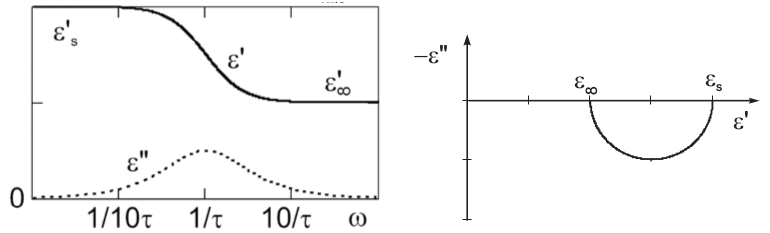
\includegraphics[scale=0.5]{ch2/image1}
\captionof{figure}{Dépendance fréquentielle de $\epsilon'$ et $\epsilon''$ pour une relaxation à gauche
et représentation Cole-Cole à droite.}
\end{center}
La réponse impulsionnelle correspondante à ce phénomène est donnée par
\begin{equation}
\epsilon(t) = \epsilon_\infty'.\delta(t) +(\epsilon_s'-\epsilon_\infty')\dfrac{e^{-t/\tau}}{\tau}
\end{equation}
Notons que les relations de Kramiers-Kronig ne sont pas vérifiée par la limite à haute-fréquence est
non-nulle (mais $\epsilon-\epsilon_\infty'$ oui).
\newpage
\item \textbf{Processus de résonance}\\
La dépendance en fréquence de la permittivité à la forme
\begin{equation}
\epsilon(\omega) = \epsilon_\infty'+(\epsilon_s'-\epsilon_\infty')\dfrac{\omega_0^2}{\omega_0^2-\omega^2
+i\omega.2\Delta}
\end{equation}
où $\omega_0$ est la pulsation de résonance et $2\Delta$ la largeur de résonance. L'équation (2.42) donne
la réponse impulsionnelle.
\begin{center}
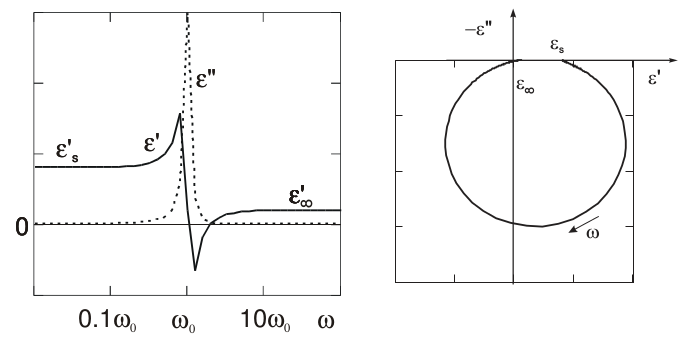
\includegraphics[scale=0.5]{ch2/image2}
\captionof{figure}{Dépendance fréquentielle de $\epsilon'$ et $\epsilon''$ pour une résonance à gauche
et représentation Cole-Cole à droite.}
\end{center}
Proche de la résonance ($|\omega-\omega_0|\ll \omega_0$), si la largeur de résonance est bien plus 
petite que la fréquence de résonance ($2\Delta \ll \omega_0$), on peut faire l'approximation que
\begin{equation}
\epsilon = \epsilon_\infty'+\dfrac{\omega_0}{2}\dfrac{\epsilon_s'-\epsilon_\infty'}{\omega_0-\omega+i\Delta}
\end{equation}
\item \textbf{Dispersion de Sellmeier}\\
L’absorption est souvent négligeable dans les régions loin de la résonance. La permittivité est 
alors approximativement réelle et la dispersion pour un processus de résonance devient
\begin{equation}
\epsilon(\omega) = \epsilon_\infty'+(\epsilon_s'-\epsilon_\infty').\dfrac{\omega_0^2}{\omega_0^2-\omega^2}
\end{equation}
S'il y a des résonances à haute ou basse fréquence, la dispersion peut être bien approximée par l'équation
de Sellmeier
\begin{equation}
\epsilon(\omega) = \epsilon_0\left(1+\sum_j\dfrac{S_j\omega_j^2}{\omega_j'^2-\omega^2}\right)
\end{equation}
\end{enumerate}

\subsection{Dispersion Formula for Refractive Index}
La dispersion sur l'indice de réfraction est bien approximée par (basée sur l'équation de Sellmeier)
\begin{equation}
n^2(\omega) = 1+\sum_j\dfrac{S_j\omega_j^2}{\omega_j'^2-\omega^2}
\end{equation}

\newpage
\section{Linear Magnetic Materials}
Le champ de magnétisation est lié au champ magnétique via
\begin{equation}
\vec M = \chi_m\vec{H}
\end{equation}
Par définition, le champ d'induction magnétique est donné par
\begin{equation}
B \equiv \mu_0(H+M) = \mu_0(1+\chi_m)H=\mu H
\end{equation}
Cependant, pour la quasi-totalité des matériaux optiques $\chi_m\approx0$. On dira alors que $\mu\approx
\mu_0$ et $B \approx \mu_0H$.

\section{Reflection}
La réflectance $R$ est donnée par\footnote{Voir TP1}
\begin{equation}
R = \dfrac{|n-1|^2}{|n+1|^2} = \dfrac{(n'-1)^2+n^{''2}}{(n'+1)^2+n^{''2}}
\end{equation}

\section{The Electromagnetic Spectrum}
Le par-cœur c'est mal, mais ça peut (vraiment) aider ici :
\begin{center}
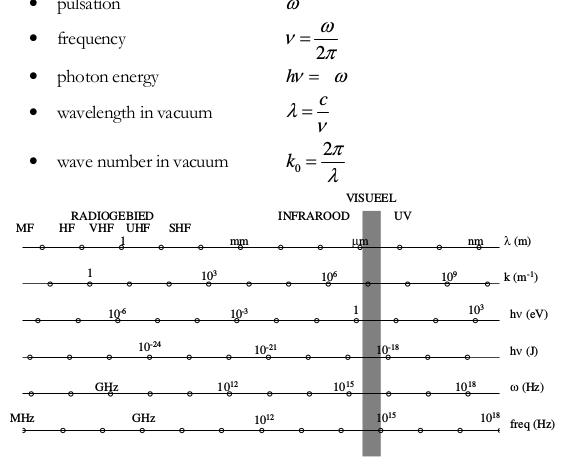
\includegraphics[scale=0.65]{ch2/image3}
\captionof{figure}{}
\end{center}
